\documentclass[a4paper,11pt]{scrartcl} %Standard A4, 11pt Font Größe
\usepackage{fullpage} %weniger Rand
\usepackage[utf8]{inputenc} %richtige Kodierung, auch für Umlaute
% \usepackage{german} %Deutsch mit Zeilenumbrüchen
% \usepackage[german]{babel}
\usepackage{latexsym} %laden von weiteren mathematischen Symbolen
\usepackage{amssymb} % mathematische Symbolzeichensätze (z.B. \mathbb{)
\usepackage{graphicx} %Figures und Subfigures
\usepackage{caption}
\usepackage{subcaption}
\usepackage[obeyspaces,hyphens]{url}
\usepackage{cite}
\usepackage{xcolor}
\usepackage{soul}
\usepackage{amsmath}
\usepackage{algorithm}% http://ctan.org/pkg/algorithms
\usepackage{algpseudocode}% http://ctan.org/pkg/algorithmicx
\usepackage{listings}
\usepackage{xcolor}
\usepackage{textcomp}
\usepackage{hyperref}

\definecolor{listinggray}{gray}{0.9}
\definecolor{lbcolor}{rgb}{0.9,0.9,0.9}

\lstset{
morekeywords={pragma},
    backgroundcolor=\color{lbcolor},
    tabsize=4,
  language=C++,
  captionpos=b,
  tabsize=3,
  frame=lines,
  numbers=left,
  numberstyle=\tiny,
  numbersep=5pt,
  breaklines=true,
  showstringspaces=false,
  basicstyle=\footnotesize,
  directivestyle={\color{red}},
%  identifierstyle=\color{magenta},
  keywordstyle=\color[rgb]{0,0,1},
  commentstyle=\color{olive},
  stringstyle=\color{red}
  }

\definecolor{lightgray}{rgb}{0.6,0.6,0.6}
\definecolor{darkgray}{rgb}{0.3,0.3,0.3}
\newcommand{\err}[1]{$^{\textcolor{red}{#1}}$}
\newcommand{\fl}[1]{\colorbox{lightgray!20}{\path{#1}}}
\newcommand{\cd}[1]{\sethlcolor{darkgray} \textcolor{white}{\hl{\texttt{#1}}}}
\newcommand*{\vv}[1]{\vec{\mkern0mu#1}}

%Header und Titel
\title{N-Body Simulation}
\subtitle{VL Parallele Systeme, HTW Berlin, SS2017}
\author{Richard Remus, Jonas Jaszkowic}
\date{}

%----------------------------------------------------------------------
\begin{document}
\maketitle
% \tableofcontents

\section{Introduction}
Implementing a N-body simulation breaks down to solving the N-body problem of predicting the individual motions of a group of $n$ objects interacting with each other gravitationally. The exact solution to this problem has a time complexity of $\mathcal{O}(n^2)$ which means that it is not possible to solve it efficiently in an appropriate period of time, especially when the number of objects is large. Reducing time complexity can either be done by using approximate methods which produce a "good enough" solution or by parallelizing the algorithm on multi-core processors. For this work, we focus on the latter.

\section{N-body problem}
The N-body problem is a generalized form of the famous two-body and three-body problem which are dealing with the same question: determining the motions of two or three bodies interacting with each other gravitationally. An explicit analytical solution is known to the two-body problem, i.e. simple functions $\vv{r_1}(t)$ and $\vv{r_2}(t)$ that takes only the time $t$ as a parameter and calculates the corresponding position of both bodies given only the initial conditions. However, up to today no analytical solution in the form of $\vv{r_i}(t)$ functions has been found for the three-body problem or the n-body problem. \cite{nbodysolve} The most straight-forward methods are called \textit{direct} methods or \textit{particle-particle} methods. For these problems, a number of numerical solutions are known.
\subsection{Definition}
The n-body problem is given by $n$ point masses $m_i > 0$ and $n$ initial position vectors $\vv{r_i}$ for $i=1,2,...,n$ in a three-dimensional reference system $\mathbb{R}^3$, their mutual gravitational attraction being the single force acting on them. \cite{meyer2008introduction}Given these initial conditions, the task can now be stated as: \textit{Find the position vectors for each body given a time $t$.}
\subsection{Derivation}
Finding the body positions boils down to calculating the acceleration for each body. Using Newton' second law of motion
\begin{align*}
F = m \cdot a
\end{align*}\\
we can state that mass times acceleration of the $i$th body is equal to the sum of the forces acting on this particular body. The sum of the forces can be calculated using Newton's universal law of gravity
\begin{align*}
F = \gamma \cdot \frac{m_1m_2}{r^2}
\end{align*}\\
where $\gamma$ is the gravitational constant, and the superposition principle
\begin{align*}
\vv{F_{res}} = \vv{F_1} + \vv{F_2} + ... + \vv{F_n}
\end{align*}\\
and the direction of this force defined by
\begin{align*}
\vv{q_j} -\vv{q_i}~/~||\vv{q_j} - \vv{q_i}||
\end{align*}
With these basic laws we can derive the acceleration $a_i$ for every body:
\begin{align*}
	m_i \cdot a_i &= F\\
	m_i \cdot a_i &= \gamma \sum\limits_{j=1}^N \frac{m_i m_j}{||\vv{q_j} - \vv{q_i}||^2}  \\
	\vec{a}^{\,}_i \cdot m_i &= \gamma \sum\limits_{j=1}^N \frac{m_i m_j}{||\vv{q_j} - \vv{q_i}||^2} \cdot \frac{(\vv{q_j} - \vv{q_i})}{||\vv{q_j} - \vv{q_i}||} \\
	\vv{a_i} &= \gamma \sum\limits_{j=1}^N \frac{m_j \cdot (\vv{q_j} - \vv{q_i})}{||\vv{q_j} - \vv{q_i}||^3}
\end{align*}\\
In order to avoid division by zero in the distance calculation $||\vv{q_j} - \vv{q_i}||$ we introduce a softening factor $\epsilon$:

\begin{align*}
	\vv{a_i} &= \gamma \sum\limits_{j=1}^N \frac{m_j \cdot (\vv{q_j} - \vv{q_i})}{(||\vv{q_j} - \vv{q_i}||^2 + \epsilon^2)^\frac{3}{2}}
\end{align*}
With this equation we have deducted the acceleration $\vv{a_i}$ of each body. Using infinitesimal time steps and the laws $v = a\cdot t$ and $s=v\cdot t$, we can iteratively calculate the postion of each body for every time $t$.

\section{Algorithm}
With the above physical equations we can formulate an algorithm for the simulation of the body positions over time given an initial configuration. This algorithm uses the \textit{direct} method and features no further optimizations beside the parallelization that is applied later on. The core algorithm consists of a nested for loop that iterates for each body $i$ over all other bodies $j$ in order to accumulate the forces acting on body $i$. It is important to note that we have to accumulate all forces \textit{before} the calculation of velocity and position can accur, otherwise the update of the position would lead to incorrect results.
\begin{algorithm}[H]
\caption{Update body positions for the given timestep $\Delta$}
\begin{algorithmic}[1]
\Procedure{UpdateStep}{$bodies$,~$\Delta$}
   \For{each body $i$ in $bodies$}
      \State $\vv{a_i} \gets 0$ \Comment{Reset forces for $i$}
      \For{each body $j \neq i$ in $bodies$}
        \State $\vv{a_i} \gets \vv{a_i} + $ CalculateForce($j,i$)
      \EndFor
   \EndFor
   \For{each body $i$}
      \State $\vv{v_i} \gets \vv{v_i} + \Delta * \vv{a_i}$ \Comment{Update velocity}
      \State $\vv{r_i} \gets \vv{r_i} + \Delta * \vv{v_i}$ \Comment{Update position}
   \EndFor
\EndProcedure\\
\Procedure{CalculateForce}{$j,~i$}
	\State \Return $\gamma \frac{m_j \cdot (\vv{q_j} - \vv{q_i})}{(||\vv{q_j} - \vv{q_i}||^2 + \epsilon^2)^\frac{3}{2}}$
\EndProcedure
\end{algorithmic}
\label{alg:core}
\end{algorithm}

Because the calculation of the force for each body is independent of previous steps or partial results the nested for-loop can be fully parallelized. The same applies for the second for-loop that updates the positions and velocities.

\section{Implementation}
The simulation and the core algorithm were implemented in \texttt{C/C++} with OpenMP \cite{openmp} and OpenCL \cite{opencl} as parallelization frameworks. For developing and debugging we used the CLion IDE \cite{clion} on two identical MacBook Pro machines running macOS Sierra. The project build specifications were managed with CMake.

Also we tried out different testing frameworks like cunit, but finally settled with \texttt{Google-Test} since it was easy to set up, updates itself on build time and has integration with the CLion IDE, which enabled us to run specific tests or test suites on demand.

We also implemented a real time visualization with Processing, a micro framework for the development of graphical applications based on the usage of a \textit{setup-and-loop} pattern. The visualization supports both a replay from a log file and realtime processing of a log stream.

The application itself supports an extensive command line interface in order to specify precise configuration of the simulator.

\subsection{Software design}
\label{software_design}
The final application is composed of a relatively small number of classes, since its only purpose is the simulation while the visualization of the simulation data was completely externalized. Nevertheless, we tried to apply fitting design patterns in order to accomplish a clean, sensible and maintainable implementation. The class hierarchy is portrayed in \cite{fig:classes} with exclusion of the main class, since it just provides configuration parsing as well instantiation of the seimulator and is not really important in regards to the simulation itself.

\begin{figure}[h!]
	\centering
	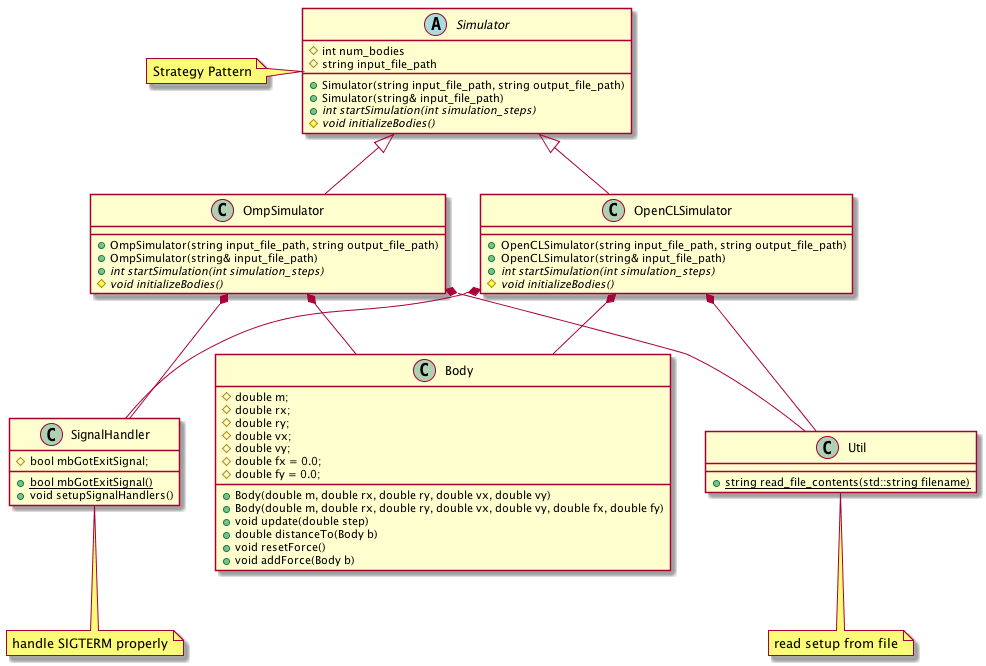
\includegraphics[width=\textwidth]{img/classes.png}
	\caption{Architectural overview of the classes involved in the simulation.}
	\label{fig:classes}
\end{figure}

Since one requirement was that we try out different parallelization approaches and we did not want to develop two applications with large sets of duplicated code, we tried to instantiate the different simulators dynamically during setup within a single application. The solution offerd itself through the application of the strategy design pattern. In other words, we encapsulated the different parallelization approaches in whithin the seperate simulator classes \texttt{OmpSimulator} and \texttt{OpenClSimulator} respectively. To gain interchangeability, both implementations suffice the abstraction which is defined in form of the class \texttt{Simulator}.

Since the setup of the simulated physical system was also exterenalized with configuration files, we had to implement a file parsing in a \texttt{Util} class.

The requirement to have a simulation run indefinitely, proved to be challenging, since the application had to support some kind of interrupt, so that objects could be cleaned up properly before shutdown. So we looked up strategies to handle system level termination signals, \texttt{SIGTERM} precisely, and found a solution which we realized in the class \texttt{SignalHandler}. Basically, an instance of \texttt{SignalHandler} checks whether a registered callback received a kill signal during every single iteration of the simulator.

The specific representation of the physical bodies is realized through the aptly named class \texttt{Body}. In this singular case, property naming deviates from clean code naming conventions and is directly adopted from the underlying mathematical nomenclature instead.

\subsection{Astronomical Units}
Distances, masses and velocities in the universe lead to large numbers that might not fit in floating
point numbers. Because many OpenCL vendors do not support double precision numbers, we scale these values to astronomical units that will fit in single precision floating points. In astronomical units, time is
measured in years, distances in AU and masses in solar-masses:

\begin{align*}
	1~yr &= 365.25 * 86400~s = 31557600~s \\
	1~AU &= 149597870700~m \\
	1~M &=  1.98892 \cdot 10^{30}~kg
\end{align*}

With these values we can scale the gravitational constant accordingly \cite{astrounits}:

\begin{align*}
	6.674 \cdot 10^{-11} \frac{m^3}{kg \cdot s^2}
	& =  6.674 \cdot 10^{-11} \cdot 2.98692\cdot 10^{-34} \frac{AU^3}{kg \cdot s^2}\\
	& = 6.674 \cdot 10^{-11} \cdot 2.98692\cdot 10^{-34} \cdot 1.98892 \cdot 10^{30} \frac{AU^3}{M \cdot s^2} \\
	& = 6.674 \cdot 10^{-11} \cdot 2.98692\cdot 10^{-34} \cdot 1.98892 \cdot 10^{30} \cdot 9.95844249\cdot 10^{14} \frac{AU^3}{M \cdot yr^2}\\
	& = 39.445 \frac{AU^3}{M \cdot yr^2}
\end{align*}

\section{Parallelization}
\subsection{OpenMP}
OpenMP (\textit{Open Multi-Processing}) is an application programming interface that enables parallelization through the use of multiple threads that are executed concurrently. OpenMP is a high-level API that lightens the user's workload with a set of simple compiler directives, library routines and environment variables that enable nearly-automatic parallelization. It is especially easy to parallelize even nested for-loops as long as some prerequisites are fulfilled. For example a simple two-dimensional for loop can be parallelized with the pragma \texttt{\#pragma omp parallel for collapse(2) \{...\}}. This leads to the creation of \texttt{OMP\_NUM\_THREADS} threads, each executing an equally large part of this loop. The environmental variable \texttt{OMP\_NUM\_THREADS} can be set to an arbitrary value before executing the code. For all practical purposes the number of threads is limited to the number of (virtual) CPUs on the machine. Setting this number to a higher value than available CPUs will \textbf{not} lead to faster execution times but in fact will slow down the execution. Therefore it is advised to set $1 \leq $ \texttt{OMP\_NUM\_THREADS} $\leq $ \texttt{NUM\_CPUs}. Listing \ref{lst:openmppar} shows the relevant part of the simulation code that can be parallelized using OpenMP. It follows the basic pattern of the core algorithm described in Algorithm \ref{alg:core} but uses an additional for loop to reset the forces. This is necessary because OpenMP only allows statements in the inner for-loop.\\

\lstinputlisting[escapeinside={\X\X}, caption={Part of the code that is parallelized using OpenMP}, label={lst:openmppar}]{omp_extract.cpp}

\subsection{OpenCL}
The \textit{Open Computing Language} (OpenCL) is a general-purpose framework for parallelization on heterogeneous platforms. It enables the processing power of CPUs and GPUs. OpenCL specifies it's own programming language \texttt{OpenCL C} that is based on \texttt{C99} and \texttt{C++}. The core concept of OpenCL is the use of so called \textit{kernels}, functions that are executed on an OpenCL device. Following the SPMD (single program, multiple data) approach, this function is applied to each \textit{work item} in parallel. When the number of \textit{compute units} (CUs) is smaller than the number of work items, the workload is equally distributed in work \textit{work groups}. The number of work items in a work group is called \textit{local size}, the total number of work items is called \textit{global size} with the property that the global size is equal to the number of work groups times the according local size. By adjusting these parameters the degree of parallelization can be adjusted, similar to setting \texttt{OMP\_NUM\_THREADS} in the OpenMP framework. The main advantage of OpenCL over OpenMP is the possibility to leverage the compute units available on the GPU. Because the GPU has far more compute units than any CPU, it is perfectly suited to achieve a high degree of parallelization. Listing \ref{lst:openclpar} shows the OpenCL kernel code used for the parallelization of the simulation.

\subsection{Sequential and parallel parts}
When analyzing parallelized software it is important to know which parts of the software can be parallelized and which parts are inevitable sequential. Following Amdahl's Law, the maximum theoretical speedup is limited by the sequential part of the program. Our simulation consists mainly of three parts:

\begin{itemize}
  \item Parsing of the configuration file
  \item Core algorithm
  \item Processing the results (Writing to log file)
\end{itemize}

Out of these parts, only the core algorithm can be fully parallelized.

\newpage
\lstinputlisting[escapeinside={\X\X}, caption={Kernel code for the OpenCL parallelization}, label={lst:openclpar}]{../kernel/core.cl}

\section{Simulation behavior}
As described in section \ref{software_design}, the initial configuration of the physical system (i.e. masses and body positions) are read from configuration files. This allows us to rapidly simulate and evaluate different scenarios without the need to build the software again. It is hard to tell whether the physical properties are simulated correctly, for example it is simply not feasible to calculate the forces by hand and using these values to write unit tests to verify the simulation. Therefore we created initial values for the simulation of the solar system with its 8 planets. The sun is set as the reference point at coordinates $\vv{p}=(0,0)$ with velocity $\vv{v}=(0,0)$. The $y$-position and horizontal velocity of all other planets are set to 0. Masses are set according to their real values. For the vertical velocity we used the \textit{mean orbital speed} as given by \cite{wikiplanets}. This setup results in a fairly stable orbital movement of the planets around the sun. We used this configuration as a proof-of-concept for each new simulation version.\\\\
More interesting configurations arised when the number of bodies increased. However, most of the randomly chosen configurations "exploded" after collapsing rapidly into the center of the system. Structures like clusters or stable orbital systems could only be observed by "zooming" into the regions of interest while replaying the simulation. Increasing the \textit{softening factor} $\epsilon$ prevents these "explosions" from happening because it is guaranteed that the bodies always have a certain distance which leads to \textit{softened} accelerations. It is important to note that increasing the softening factor yields \textit{unrealistic} behavior. However this does not have to be a bad thing because the simulation could also be used to generate visually appealing image sequences or general-purpose particle systems where realism is less important. Example renderings from the simulation with 2048 bodies are given in figure \ref{fig:simulation_rendering}.

\begin{figure}[tb]
  \centering
  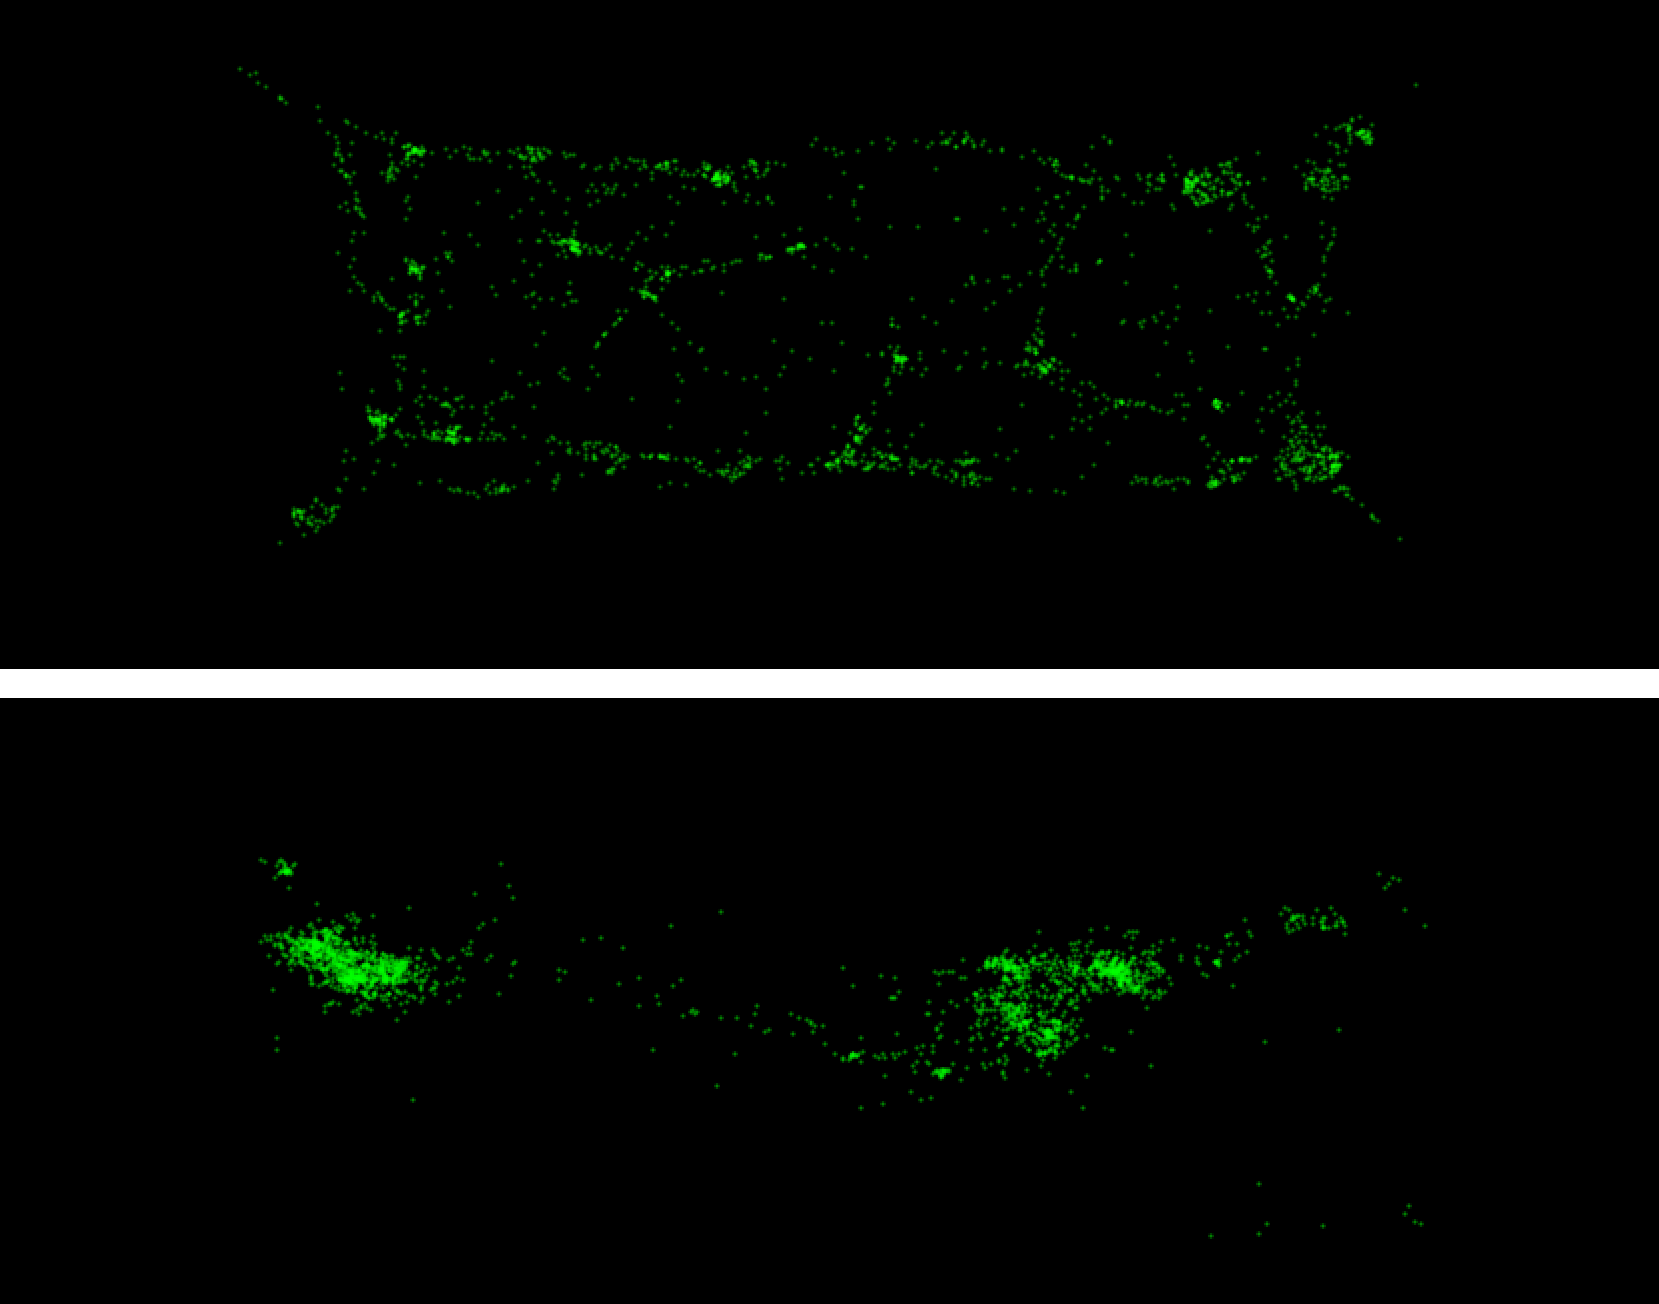
\includegraphics[width=\textwidth]{img/simulation.png}
  \caption{Simulation with 2048 bodies initially randomly placed in space with equal masses, no initial velocity and softening factor $\epsilon = 1$. Images taken after 40 and 175 simulation steps (1 simulation step equals 1 day).}
  \label{fig:simulation_rendering}
\end{figure}

\section{Benchmarks}
\subsection{Sequential vs. OpenMP vs. OpenCL}
In order to compare the three implementation types \textit{Sequential}, \textit{OpenMP} and \textit{OpenCL} we performed benchmark tests with a fixed number of simulation steps and varying number of bodies. Since the sequential part of the program is always the same in each of the different implementations, the overall execution time is a good indicator for the efficiency of the parallelization. Execution environment was a MacBook Pro with 2,7 GHz Intel Core i5 processor with 4 hyperthreaded cores and Intel Iris Graphics 6100 with a total number of 48 compute units. Based on the number of cores and compute units, the speedup $S$ was predicted to be $S=4$ for the OpenMP implementation and $S=48$ for the OpenCL implementation with the sequential implementation as a reference point.\\

\renewcommand{\arraystretch}{1.3}
\begin{table}[h!]
  \begin{tabular}{l|rrrr}
    & Execution Time (s) & Standard Deviation &  Actual Speedup & Predicted Speedup \\ \hline
    Sequential & $19342.50$ & $57.87$ & - & -\\
    OpenMP & $6557.75$ & $31.30$ & $2.95$ & $4$\\
    OpenCL & $983.63$ & $23.75$ & $19.67$ & $48$
  \end{tabular}  
  \caption{Speedup comparison: actual and predicted speedup differ significantly.}
  \label{table:speedup}
\end{table}

Table \ref{table:speedup} and figure \ref{fig:benchmark_compare} reveal that the maximum speedup of $S\approx 20$ was reached with the OpenCL implementation. However, predicted and actual speedup times differ significantly. This can be due to different background processes simultaneously running on the machine that take up computing resources. Another possible explanation is the overhead that arises from copying the required memory back and forth to the GPU or the general overhead from splitting the global task into subtasks.
\begin{figure}[h!]
  \centering
  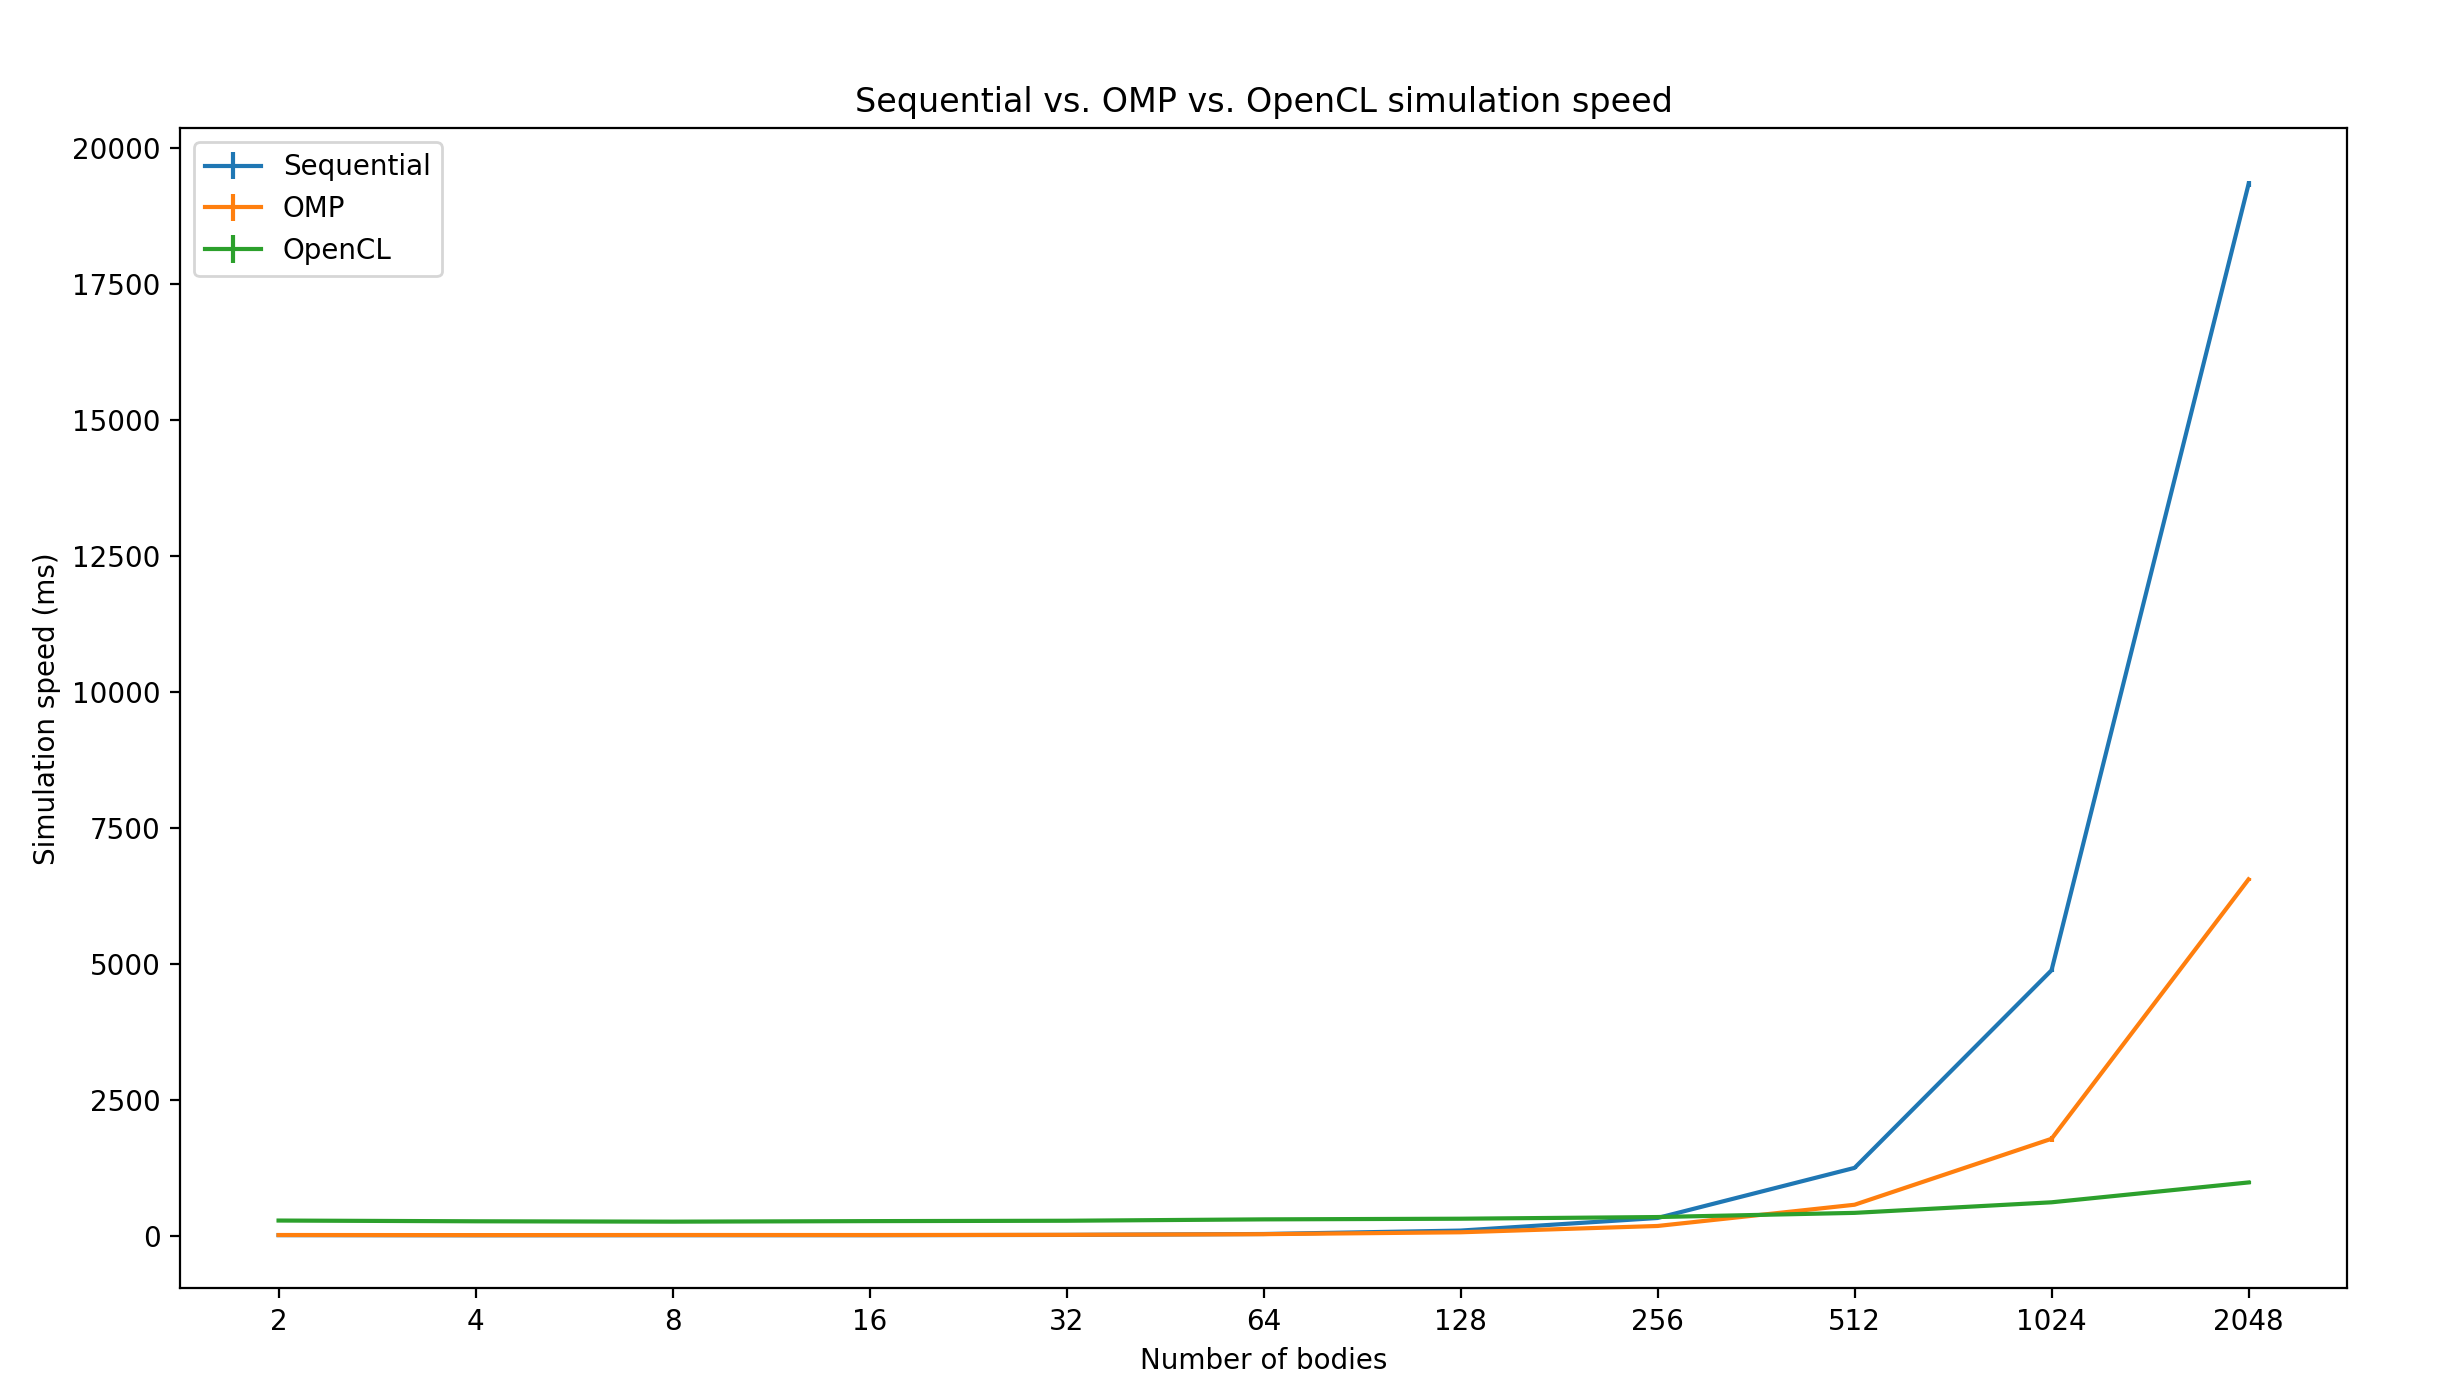
\includegraphics[width=\textwidth]{img/benchmark_compare.png}
  \caption{Comparison of the simulation speeds of the different implementation types \textit{Sequential}, \textit{OpenMP} and \textit{OpenCL}. Standard deviation over 8 runs is displayed but barely visible.}
  \label{fig:benchmark_compare}
\end{figure}

\subsection{OpenMP threads}
\begin{figure}[h!]
  \centering
  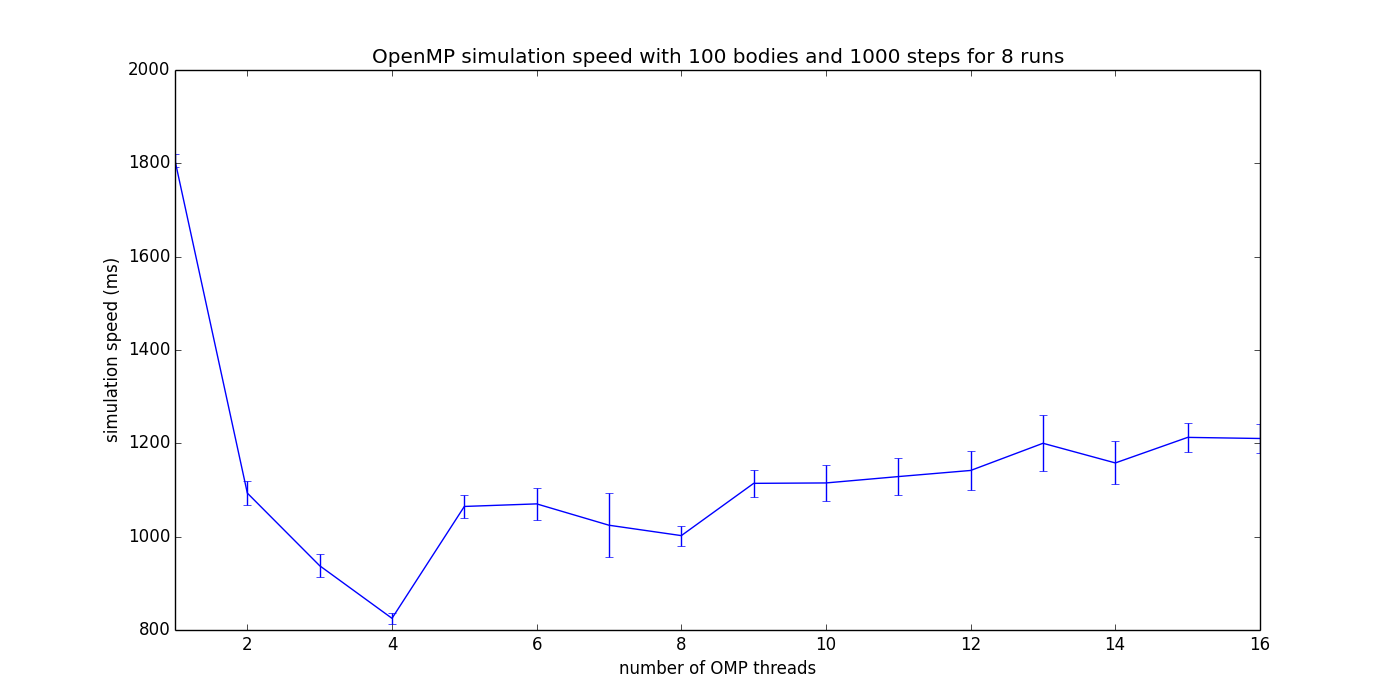
\includegraphics[width=\textwidth]{img/benchmark_omp.png}
  \caption{Simulation speed of OpenMP implementation for various number of threads. Standard deviation over 8 runs is displayed.}
  \label{fig:figure1}
\end{figure}

\section{Discussion}

\newpage
\bibliography{bibliography}{}
\bibliographystyle{plainurl}
\end{document}
